\documentclass[conference]{IEEEtran}
\IEEEoverridecommandlockouts
% The preceding line is only needed to identify funding in the first footnote. If that is unneeded, please comment it out.
\usepackage{cite}
\usepackage{amsmath,amssymb,amsfonts}
\usepackage{algorithmic}
\usepackage{graphicx}
\usepackage{textcomp}
\usepackage{xcolor}
\usepackage{hyperref}
\def\BibTeX{{\rm B\kern-.05em{\sc i\kern-.025em b}\kern-.08em
    T\kern-.1667em\lower.7ex\hbox{E}\kern-.125emX}}
\begin{document}

\title{Real-time Domain Adaptation in Semantic Segmentation*\\
{\footnotesize \textsuperscript{*}Note: Sub-titles are not captured in Xplore and
should not be used}
}

\author{\IEEEauthorblockN{1\textsuperscript{st} Berardo Nicholas}
\IEEEauthorblockA{\textit{dept. Computer Engineering} \\
\textit{Politecnico di Torino}\\
Turin, Italy \\
s319349@studenti.polito.it}
\and
\IEEEauthorblockN{2\textsuperscript{nd} Cardona Riccardo}
\IEEEauthorblockA{\textit{dept. Computer Engineering} \\
\textit{Politecnico di Torino}\\
Turin, Italy \\
s319441@studenti.polito.it}
\and
\IEEEauthorblockN{3\textsuperscript{rd} De Marco Alessando}
\IEEEauthorblockA{\textit{dept. Computer Engineering} \\
\textit{Politecnico di Torino}\\
Turin, Italy \\
sXXXXXX@studenti.polito.it}
}

\maketitle

\begin{abstract}
We use an efficient structure named Short-Term Dense Concatenate network (STDC network) for the semantic segmentation task. This
structure reduce the dimension of feature maps and use the aggregation of them for image representation, then use a Detail aggregation
module for producing the low-level features. Finally these two are merged to produce the segmentation result. We test this model on 
Cityscapes and GTA V, following the evaluation of the domain shift between GTA V and Cityscapes and finally we implement and 
unsupervised adversarial domain adaptation method used for reducing the domain shift. We also show the result for the STDC network in
term of mIoU and the result for the domain adaptation. 
\end{abstract}


\section{Introduction}
Semantic Segmentation is a topic in computer vision that aims at assigning a label to each pixel of the image. This is used in many fields
such as autonomous vehicle, video surveillance and robot sensing. There are a lot of models that can achive good accuracy. For real-time
semantic segmentation some models choose lightweight backbones for having an increase of performance but a drastic drop of accuracy. For
this reason some new methods were investigated, like feature fusion or aggregation modules. Other models reduce the input image size 
but this can result in a bad accuracy around boundaries and small object. 

STDC net \cite{b1} uses the first approach. Fig.~\ref{fig:stdc_net} shows how the image is encoded in different scales. The kernel size is also reduced
to speed-up the performance but with an acceptable loss in accuracy. Then a Detail Guidance is used to learn the space details insted of 
using a Spacial Path as in BiSeNet \cite{b2}.

The next step is domain adaptation. A model trained on a certain dataset may not generalize on an unseen dataset ending in poor performance.
This is caused by the domain shift between the source (training) and target (test) dataset, for example different cities, weather and
lighting conditions. Domain adaptation methods are used to close the gap between source and target domains. In this paper we use an 
adversarial domain adaptation method \cite{b3} composed of a segmentation model to predict the output and a discriminator to
predict is the input is from the source or target domain. The goal is to generate a segmentation output from the segmentation part that 
fool the discriminator, meaning that the segmentation output is similar between source and target domains. We show experiments done on 
the adaptation between GTAV and Cityscapes.

Our contributions can be summarized as follows:
First we build the STDC network and train it on Cityscapes and test it again on Cityscapes. Second we reply the same idea over the 
GTAV dataset, so train on GTAV and test on GTAV. Third we compute the domain shift between GTAV (source) and Cityscapes (target) domains
firstly in vanilla, then with some augmentation on GTAV. Fourth we implement the adversarial domain adaptation method and test it 
with GTAV as source domain and Cityscapes as target domain. Lastly we apply some real-time semantic segmentation method to our 
discriminator function to make it faster.

Here a look to our implementation: \url{https://github.com/Riden15/Real-time-Domain-Adaptation-in-Semantic-Segmentation}

\begin{figure}[tp]
\centerline{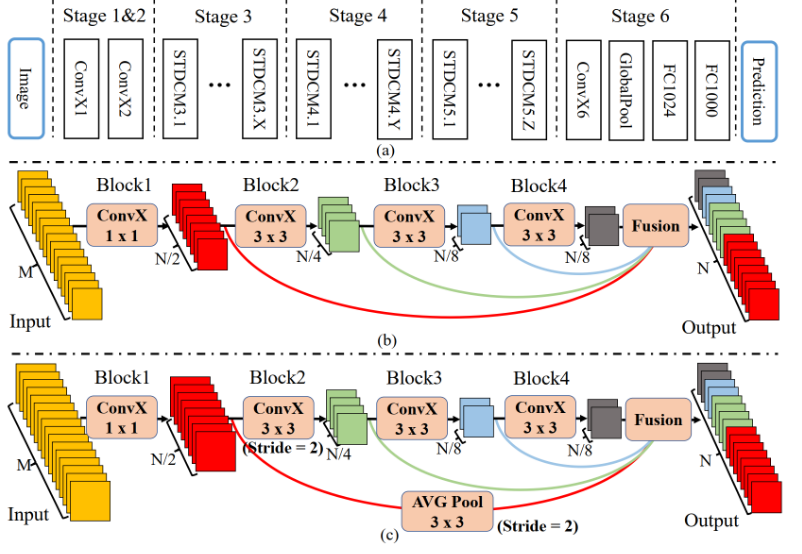
\includegraphics[width=0.4\textwidth]{figures/Figure1-STDCnet}}
\caption{STDC network.}
\label{fig:stdc_net}
\end{figure}

\section{Related Word}

\subsection{Real Time Semantic Segmentation}
parlare di bisenet e stdc, e altri metodi per semantic segmentation
\subsection{Domain Adaptation}
parlare di alcune domain adaptation method
\subsection{MobileNets}
parlare di mobilenets, come lo usiamo 
\section{Methods}

We first introduce the Short-Term Dense Concatenate network (STDC network) and how we used it with BiSeNet \cite{b2},
then the unsupervised adversarial domain adaptation method.

\subsection{Short-Term Dense Concatenate Network}

STDC network \cite{b1} is represented in Fig.~\ref{fig:stdc_net} (a). Stage 3,4 and 5 have a number of Short-Term Dense Concatenate Module (STDCM)
where each module is composed of ConvX blocks Fig.~\ref{fig:stdc_net} (b)(c). Each \(ConvX_i\) is a block composed of one convolutional layer,
one batch normalization layer and one ReLU activation layer. The ConvX layers filter the input into N/2, where N is the channel number
of the STDC module. At the end we concatenate the output of each ConvX block as follow: 
\[x_{output} = F(x_1,x_2,\dots,x_n)\]
where \(x_{output}\) is the STDC module output, \(F\) is the fusion operation, that in our case is the concatenation and \(x_1,x_2,
\dots,x_n\) are the output of each \(ConvX_i\) block.

\begin{figure}[tp]
\centerline{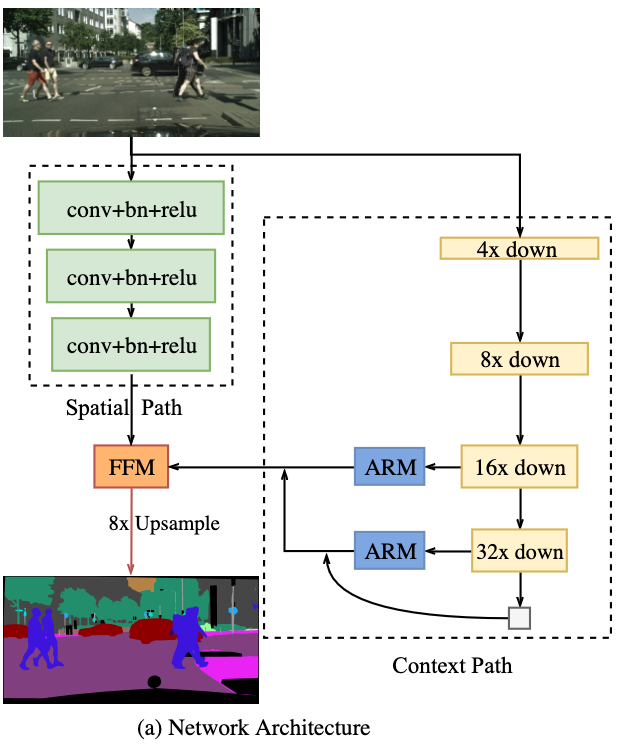
\includegraphics[width=0.4\textwidth]{figures/BiSeNet.pdf.png}}
\caption{BiSeNet network.}
\label{fig:bisenet}
\end{figure}

\subsection{BiSeNet}

BiSeNet network is represented in Fig.~\ref{fig:bisenet}. It is mainly composed of two part: Spacial Path and Context Path. 

\textbf{Spacial Path}.
Some models for real-time semantic segmentation decide to give as input a smaller image to increase the performance, but this reduce the Spacial
information of the original image resulting in a drop of accuracy. Others use lightweight models, but the spacial information is again
lost during the channel pruning. The Spacial Path that is used in BiSeNet is composed of three blocks each containing a convolution
with stride = 2, one batch normalization and ReLU activation function. This extracts a feature map that is 1/8 of the original image and
keeps a lot of spacial infromation. 

\textbf{Context Path}.
This STDC network is then used as backbone for the context path of BiSeNet, in particular we use stage 3,4 and 5 to reduce the 
feature map to obtain large receptive field. Then a global avarage pooling in added on the tail of the context path. We also use
Attention Refine Module (ARM) on Stage 4 and 5. Finally a Future Fusion Model (FFM) is used to fuse the 1/8
features from the spacial path with this last part.

\textbf{Attention Refine Module}
\begin{figure}[tp]
\centerline{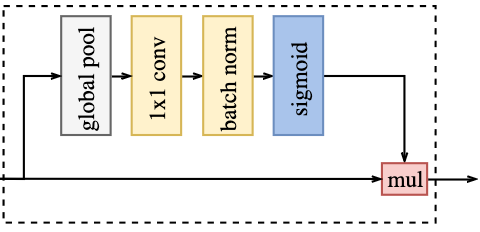
\includegraphics[width=0.4\textwidth]{figures/ARM.pdf.png}}
\caption{Attention Refine Module}
\label{fig:arm}
\end{figure}

Fig.~\ref{fig:arm} represent the Attention Refine Module (ARM). This is used in the Context Path and refines the feature of the last
two stages. It uses a global avarage pooling that capture the global context and computes an attention vector to guide the feature learning.

\textbf{Future Fusion Model}

Fig.~\ref{fig:ffm} represent the Future Fusion Model (FFM). This fuse the output of the Context Path, given by the STCD network with 
the output of the Spacial Path. The main problem of fusing these two path is that they have two different level of representation. The
Context Path represent the context information, meanwhile the Spatial Path represent the spatial information so we can't just sum them
up. Figure.~\ref{fig:ffm} shows the datails. 

\begin{figure}[tp]
\centerline{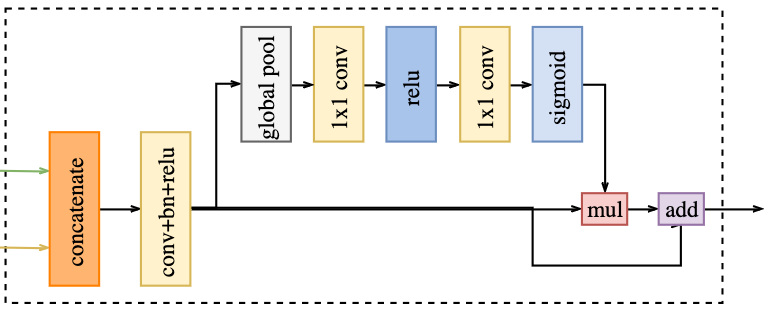
\includegraphics[width=0.4\textwidth]{figures/FFM.pdf.png}}
\caption{Future Fusion Model}
\label{fig:ffm}
\end{figure}

\subsection{Adversarial Domain Adaptation}

The main idea of the unsupervised adversarial domain adaptation method \cite{b3} is to create a segmentation network that classify the source
image (that as a label) and the target image (without annotations). Then those two predictions are given to the discriminator that
has to distinguish whether the input is from source or target domain. To do so we need a loss from the discriminator to the 
segmentation network which encourage the segmentation to generate similar predictions. We use as segmentation newtork the BiSeNet
developed above. The loss is 
\[L(I_s,I_t) = L_{seg}(I_s) + \lambda_{adv}*L_{adv}(I_t)\]
where \(L_{seg}\) is the cross entropy loss for the prediction of the source domain, \(\lambda_{adv}\) is the weight used to 
balance the \(L_{adv}\) that is a BCEWithLogitLoss.
We first forward \(I_s\) to the segmentation network to get the prediction \(P_s\) and the loss \(L_{seg}\) using the label of \(I_s\).
Then forward \(I_t\) to the segmentation network to get the prediction \(P_t\) and feed \(P_s\) to the discriminator and get the
\(L_{adv}\) and optimize the segmentation network. Now let's optimize the discriminator computing first the loss on the GTA5 image
with label 1 and finally computing the loss on the Cityscape image, with label 0. 

Finally we also tried to apply some real-time semantic segmentation method to our discriminator to make is lighter and faster.
We build a discriminator using depthwise separable convolutions, following MobileNets \cite{b6}. These are composed of two part: 
depthwise convolutions and pointwise convolutions. Depthwise convolutions are used to filter each input channel, but they can
only filter so we use pointwise convolutions (1 x 1 kernel size) to generate new features. Now our discriminator is based on blocks of
depthwise convolution layer, leaky ReLU, pointwise convolution and again leaky ReLU.

\section{Experiments}

\begin{figure}[tp]
\centerline{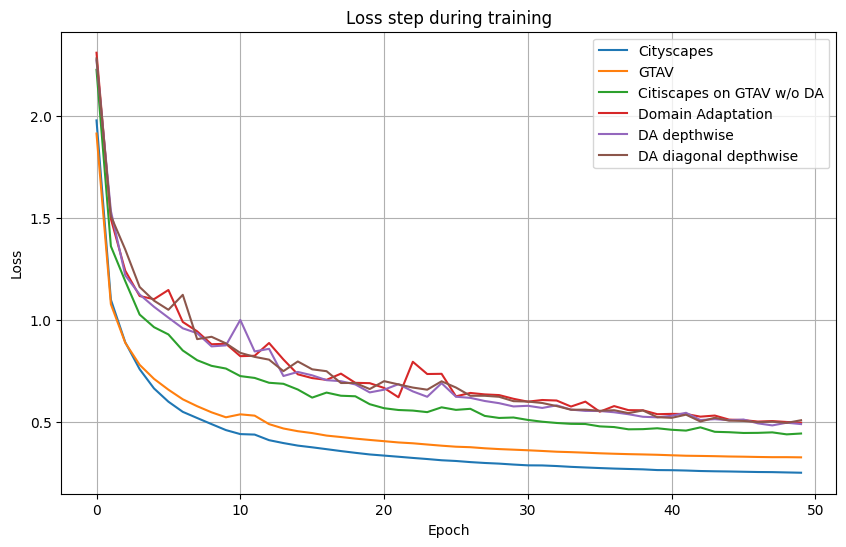
\includegraphics[width=0.4\textwidth]{figures/loss}}
\caption{Loss step during training. On the X we have the epochs, on Y we have the loss. (1) is the gray curve, (2) is the light blue
curve, (3) is the light blue curve again, (4) is the pink curve, (5) is the orange curve and (6) is the purple curve.}
\label{loss_steps}
\end{figure}

\begin{figure}[tp]
\centerline{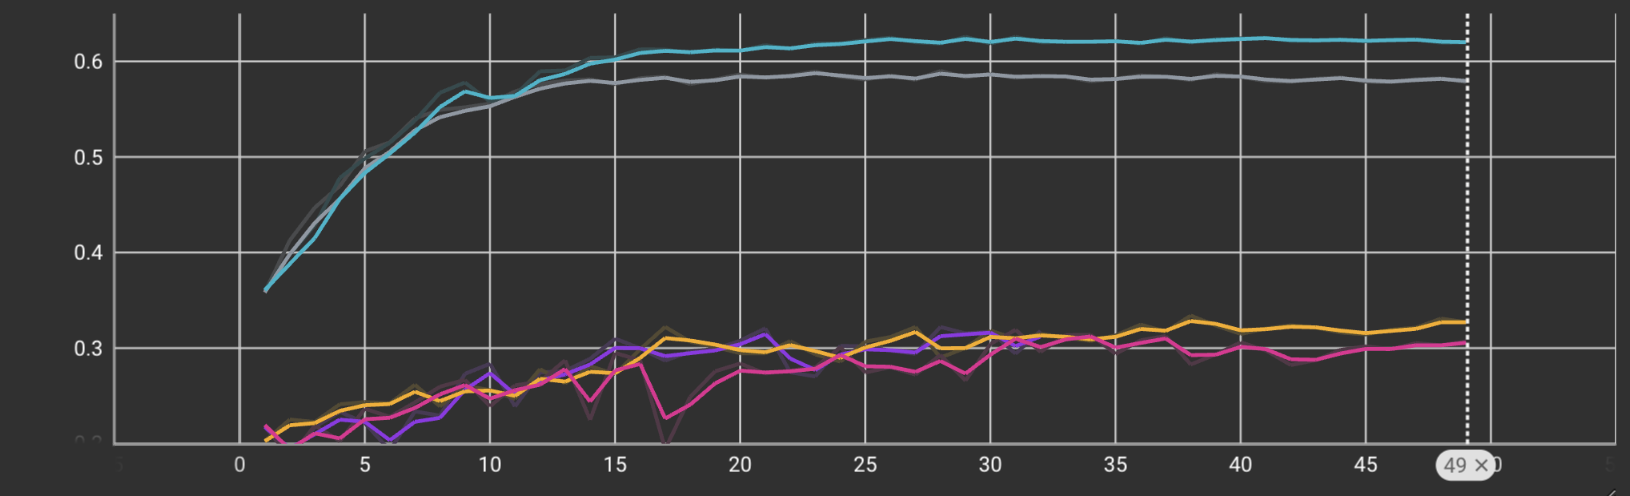
\includegraphics[width=0.4\textwidth]{figures/miou}}
\caption{mIoU during training. On the X we have the epochs, on Y we have the mIoU. (1) is the gray curve, (2) is the light blue
curve, (4) is the pink curve, (5) is the orange curve and (6) is the purple curve.}
\label{miou}
\end{figure}

\begin{figure}[tp]
\centerline{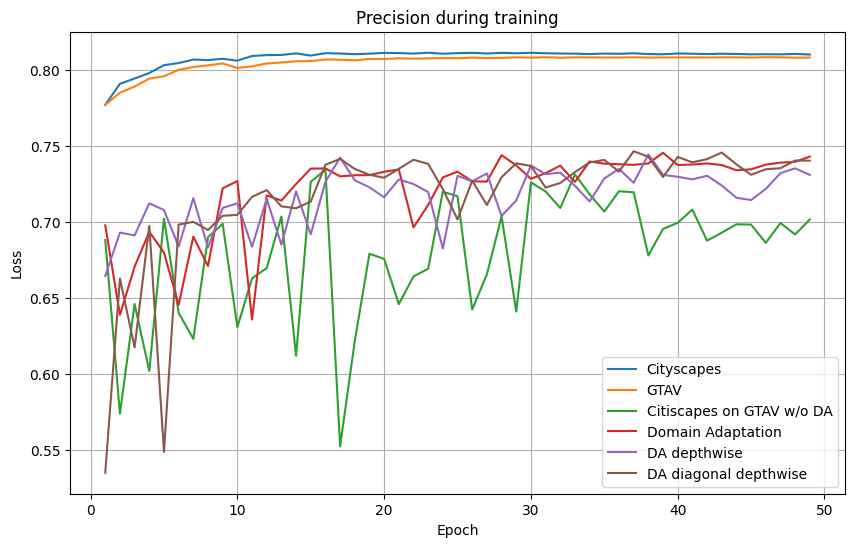
\includegraphics[width=0.4\textwidth]{figures/precision}}
\caption{Precision during training. On the X we have the epochs, on Y we have the precision. (1) is the gray curve, (2) is the light blue
curve, (4) is the pink curve, (5) is the orange curve and (6) is the purple curve.}
\label{precision}
\end{figure}

\subsection{GTA5}
GTA5 dataset \cite{b4} is composed of around 25K images with resolution 1914 x 1052 synthesized from the videogame based on Los Angeles.
The dataset is also composed of the ground truth annotation for semantic segmentation. It is based on 19 categories, that are the same
as in Cityscapes, so they are compatible. We use this dataset firstly for evaluating out model alone, so train and test on this dataset
(obviusly the test data is not seen during training). Then this dataset is used as source domain in domain adaptation.
\subsection{Cityscapes}
Cityscapes dataset \cite{b5} is composed of 5000 fine annotated images, split into training, validation and test sets with 2975, 500
and 1525 images respectively. The totale number of classes is 30, but only 19 are used for semantic segmentation. The resolution of the
images is 2048 x 1024, this is very high resolution, in fact we reduced it to 1024 x 512. This dataset is first used for evauating our
model alone, so train and test both on this dataset, then it is used as target domain for domain adaptation. 
\subsection{Experiments results}

We have done the following experiments: (1) train on Cityscapes and test on Cityscapes, (2) train on GTA5 and test on GTA5, (3) train on 
GTA5 and test on Cityscapes without domain adaptation, (4) train on GTA5 and test on Cityscapes without domain adaptation with some
augmentation on GTA5, (5) train on GTA5 and test on Cityscapes with domain adaptation and (6) train on GTA5 and test on Cityscapes with
domain adaptation with a lighter discriminator. 
We use as optimizer the SGD (Stochastic Gradient Descent) with momentum set at 0.9 and weight decay at \(5e^{-4}\). We use a batch size of
2 and poly learning rate where the learning rate is updated as follow \(lr = init\_lr * (1 - \frac{iter}{max\_iter})^{power}\), where
\(init\_lr\) is 0.01, \(iter\) is the actual epoch, \(max\_iter\) is the number of epochs and \(power\) is 0.9. Data augmentation, when
used, contains Color Jitter, Random Horizontal Flip, Random Crop and Normalization. The disciminator for the domain apadtation part
is trained using Adam with a poly learning rate with the same parameter as before. 
We perform our experiments with those versions:\textbf{TODO!!!!!!!!!}

In Fig.~\ref{loss_steps} we can see the loss step during train time. The one that can achive a better low (lower) are the experiments
where there isn't a domain shift. Same thing happend with the mean Intersection over Union (mIoU) in Fig.~\ref{miou} and with the
precision in Fig.~\ref{precision}. 

(1) Here we train our model on Cityscapes train set and test it on Cityscapes validation set. Here there's no domain adaptation, so
we expect to have high results. Table~\ref{CityscapesToCityscapes} shows the results.

(2) We train our model on GTA5 train set and test it on GTA5 validation set. Again we expect high results.  
Table~\ref{GTATOGTA} shows the results.

(3) Here we evaluate the domain shift between GTA5 and Cityscapes. We train on GTA5 train set and test on Cityscapes validation set.
Here we don't have any domain adaptation method, so we expect bad results. Table~\ref{GTATOCITYSCAPESNOADAP} shows the results. We can 
see that the mIoU is low, this because the source domain and target domain are different. 

(4) Again we evaluate the domain shift between GTA5 and Cityscapes, but this time with some augmentation on GTA5. Table~\ref{GTATOCITYSCAPESNOADAPAUG}
shows the results and again the mIoU is low because of the domain shift, but higher than step (3). This thanks to the augmentation
done on GTA5.

(5) Here we have domain adaptation \cite{b3}. So we train on GTA5 and test on Cityscapes, but this time we train also the discriminator
with the segmentation network. Table~\ref{GTATOCITYSCAPESADAP} shows the results. We can see a slight improvement of performance
in the mIoU of 3\% with respect to (4).

(6) Finally we implement depthwise separable convolutions in the discriminator. Again same thing as (5) but with a lighter discriminator. Table
~\ref{GTATOCITYSCAPESADAPLIGHT} shows the results. 



\begin{table}[tb]
\caption{Train on Cityscapes train set and test it Cityscapes val set}
\begin{center}
\begin{tabular}{|c|c|c|}
\hline
\multicolumn{3}{|c|}{\textbf{Cityscapes -$>$ Cityscapes}} \\
\cline{1-3} 
\textbf{\textit{Accuracy (\%)}}& \textbf{\textit{mIoU (\%)}}& \textbf{\textit{Train time (avg per-epoch)}} \\
\hline
81.1& 58.6& 2.3 minutes   \\
\hline
\end{tabular}
\label{CityscapesToCityscapes}
\end{center}
\end{table}

\begin{table}[tb]
\caption{Train on GTA5 train set and test it GTA5 val set}
\begin{center}
\begin{tabular}{|c|c|c|}
\hline
\multicolumn{3}{|c|}{\textbf{GTA5 -$>$ GTA5}} \\
\cline{1-3} 
\textbf{\textit{Accuracy (\%)}}& \textbf{\textit{mIoU (\%)}}& \textbf{\textit{Train time (avg per-epoch)}} \\
\hline
80.8& 62.3& 3.2 minutes   \\
\hline
\end{tabular}
\label{GTATOGTA}
\end{center}
\end{table}

\begin{table}[tb]
\caption{Train on GTA5 train set and test it Cityscapes val set without adaptation}
\begin{center}
\begin{tabular}{|c|c|c|}
\hline
\multicolumn{3}{|c|}{\textbf{GTA5 -$>$ Cityscapes}} \\
\cline{1-3} 
\textbf{\textit{Accuracy (\%)}}& \textbf{\textit{mIoU (\%)}}& \textbf{\textit{Train time (avg per-epoch)}} \\
\hline
60.1 & 24.6 & 3.2 minutes \\
\hline
\end{tabular}
\label{GTATOCITYSCAPESNOADAP}
\end{center}
\end{table}

\begin{table}[tb]
\caption{Train on GTA5 augemnted train set and test it Cityscapes val set without adaptation}
\begin{center}
\begin{tabular}{|c|c|c|}
\hline
\multicolumn{3}{|c|}{\textbf{GTA5 -$>$ Cityscapes}} \\
\cline{1-3} 
\textbf{\textit{Accuracy (\%)}}& \textbf{\textit{mIoU (\%)}}& \textbf{\textit{Train time (avg per-epoch)}} \\
\hline
71 & 30 & 5.37 minutes \\
\hline
\end{tabular}
\label{GTATOCITYSCAPESNOADAPAUG}
\end{center}
\end{table}

\begin{table}[tb]
\caption{Train on GTA5 augemnted train set and test it Cityscapes val set with adaptation}
\begin{center}
\begin{tabular}{|c|c|c|}
\hline
\multicolumn{3}{|c|}{\textbf{GTA5 -$>$ Cityscapes}} \\
\cline{1-3} 
\textbf{\textit{Accuracy (\%)}}& \textbf{\textit{mIoU (\%)}}& \textbf{\textit{Train time (avg per-epoch)}} \\
\hline
74 & 33 & 4.30 minutes \\
\hline
\end{tabular}
\label{GTATOCITYSCAPESADAP}
\end{center}
\end{table}

\begin{table}[tb]
\caption{Train on GTA5 augemnted train set and test it Cityscapes val set with lighter adaptation}
\begin{center}
\begin{tabular}{|c|c|c|}
\hline
\multicolumn{3}{|c|}{\textbf{GTA5 -$>$ Cityscapes}} \\
\cline{1-3} 
\textbf{\textit{Accuracy (\%)}}& \textbf{\textit{mIoU (\%)}}& \textbf{\textit{Train time (avg per-epoch)}} \\
\hline
73& 32.5& 4.25 minutes\\
\hline
\end{tabular}
\label{GTATOCITYSCAPESADAPLIGHT}
\end{center}
\end{table}

\section{Conclusion}

In this paper we build a model based on BiSeNet \cite{b2} with a Short-Term Dense Concatenate network (STDC network) \cite{b1} as Context Path, 
based on different STDC modules. Then we implement an adversarial domain adaptation mathod \cite{b3} to reduce the domain shift between GTA5
and Cityscapes. From the experiments we can see that having a domain adaptation method can help in increasing the accuracy and mIoU. 
Finally we develop a lighter and faster method for discriminate the source and target data in the domain adaptation
method, based on MobileNets \cite{b6}. 

\section*{Acknowledgment}

The preferred spelling of the word ``acknowledgment'' in America is without 
an ``e'' after the ``g''. Avoid the stilted expression ``one of us (R. B. 
G.) thanks $\ldots$''. Instead, try ``R. B. G. thanks$\ldots$''. Put sponsor 
acknowledgments in the unnumbered footnote on the first page.

\section*{References}

\begin{thebibliography}{00}
\bibitem{b1} Mingyuan Fan, Shenqi Lai, Junshi Huang, Xiaoming Wei, Zhenhua Chai, Junfeng Luo, Xiaolin Wei. Rethinking BiSeNet For Real-time Semantic Segmentation. 2021
\bibitem{b2} Changqian Yu, Jingbo Wang, Chao Peng, Changxin Gao, Gang Yu, and Nong Sang. Bisenet: Bilateral segmentation network for real-time semantic segmentation. In European conference on computer vision (ECCV) 2018.
\bibitem{b3} Yi-Hsuan Tsai, Wei-Chih Hung, Samuel Schulter, Kihyuk Sohn, Ming-Hsuan Yang, Manmohan Chandraker. Learning to Adapt Structured Output Space for Semantic Segmentation. In CVPR, 2018
\bibitem{b4} S. R. Richter, V. Vineet, S. Roth, and V. Koltun. Playing for data: Ground truth from computer games. In ECCV, 2016.
\bibitem{b5} M. Cordts, M. Omran, S. Ramos, T. Rehfeld, M. Enzweiler, R. Benenson, U. Franke, S. Roth, and B. Schiele. The cityscapes dataset for semantic urban scene understanding. In CVPR, 2016. 
\bibitem{b6} Andrew G. Howard, Menglong Zhu, Bo Chen, Dmitry Kalenichenko, Weijun Wang, Tobias Weyand, Marco Andreetto, Hartwig Adam. MobileNets: Efficient Convolutional Neural Networks for Mobile Vision Applications. 2017
\end{thebibliography}
\vspace{12pt}

\end{document}
